% LREC 2026 Paper: Controlling Text Complexity in Small Language Models
\documentclass[10pt, a4paper]{article}

\usepackage[review]{lrec2026}

\title{Controlling Text Complexity in Small Language Models for A1 English Learners: \\ Comparing Prompting and Probability Weighting Strategies}

\name{Author1, Author2, Author3} 

\address{Affiliation1, Affiliation2, Affiliation3 \\
         Address1, Address2, Address3 \\
         author1@xxx.yy, author2@zzz.edu, author3@hhh.com\\}


\abstract{
Language learning applications require AI assistants that can adapt their complexity to match learner proficiency levels. We investigate two lightweight, inference-time interventions for controlling text complexity in small language models (0.5B-3.8B parameters): context prompting and probability weighting. Through a factorial experiment across 6 models (Phi3, Qwen2, Qwen3, SmolLM, TinyLlama, TinyStories) with 4 configurations and 8 prompts (192 total observations), we evaluate their effectiveness using 18 readability metrics. Our results show [TBD: key findings pending full experiments]. This work represents the first systematic comparison of inference-time complexity control methods for small models in educational contexts, providing practical guidelines for deploying language learning assistants.
\\ \newline \Keywords{text simplification, small language models, controllable generation, language learning, educational NLP, readability assessment, CEFR}}

\begin{document}

\maketitleabstract

\section{Introduction}

Language learning applications increasingly rely on conversational AI to provide personalized support to learners. However, a critical challenge remains: ensuring that AI-generated responses match the learner's proficiency level. An A1-level English learner (CEFR beginner) with a vocabulary of approximately 500 words requires fundamentally different language than an advanced learner.

Consider the following example from our experiments:

\begin{quote}
\textbf{Prompt:} ``What does the word `library' mean?''

\textbf{Control (Qwen2, no interventions):} \\
``The word `library' means a collection of books, magazines, and other printed materials organized and maintained by a library staff...'' \\
→ Flesch-Kincaid Grade: 11.5 | Too complex for A1!

\textbf{Both interventions (Qwen2):} \\
``A library is a place where you can find lots of books to read. It's like a big house with many special rooms where people keep their toys and stories!'' \\
→ Flesch-Kincaid Grade: 5.8 | A1-appropriate!
\end{quote}

Small language models (SLMs) offer significant advantages for educational deployment: on-device processing, low latency, privacy preservation, and reduced computational costs \citep{TBD}. However, SLMs trained on general-domain corpora typically produce text too complex for beginner learners \citep{TBD}.

Traditional approaches to text simplification either apply post-hoc rewriting \citep{Gala2018,Crossley2011} or require resource-intensive fine-tuning on labeled data \citep{Al-Thanyyan2020,Baez2023}. Recent work on controllable generation has explored fine-tuning with complexity values \citep{Nguyen2024} and activation engineering \citep{Zhang2025}, but these approaches target large models (7B+ parameters) and require additional training.

\textbf{Our contribution:} We investigate two lightweight, inference-time interventions applicable to any pre-trained small language model without additional training:

\begin{enumerate}
\item \textbf{Context Prompting:} System-level instructions to simplify language
\item \textbf{Probability Weighting:} Logits manipulation to boost A1 vocabulary tokens
\end{enumerate}

Through a factorial design across 6 models (33M to 3.8B parameters), we address the following research questions:

\begin{enumerate}
\item How effective is each intervention at reducing text complexity?
\item Do combined interventions produce synergistic effects?
\item What are the trade-offs between complexity reduction and response time?
\item Which small models are best suited for educational deployment?
\end{enumerate}

Our systematic evaluation using 18 readability metrics across 192 observations provides the first comprehensive comparison of inference-time complexity control for small language models in educational contexts.

\section{Related Work}

\subsection{Text Simplification for Language Learning}

Empirical studies demonstrate that simplified texts improve reading comprehension, particularly for beginning readers \citep{Gala2018} and second language learners \citep{Crossley2011}. Traditional approaches focus on lexical substitution (replacing difficult words) and syntactic simplification (shortening sentences) \citep{Claridge2005}.

Recent neural approaches have explored readability-controlled generation. \citet{Al-Thanyyan2020} trained models on the Newsela corpus to produce text at specific grade levels, while \citet{Al-Sabbagh2023} reviewed multi-level simplification systems across languages. However, these approaches require training on labeled parallel corpora and lack flexibility to adjust complexity dynamically.

\subsection{Controllable Text Generation}

\textbf{Fine-tuning approaches:} \citet{Nguyen2024} introduced Multi-Control Tuning (MCTune), which fine-tunes LLaMA2-7B by incorporating linguistic complexity values during instruction tuning. This achieves precise control over multiple complexity dimensions but requires substantial computational resources and locks the model to specific complexity levels learned during training. \citet{Baez2023} similarly fine-tuned LLaMA for lexical simplification, demonstrating baseline performance but facing similar resource constraints.

\textbf{Activation engineering:} \citet{Zhang2025} proposed Generation with Concept Activation Vector (GCAV), which trains concept activation vectors for attributes like toxicity and adjusts them during inference. While this avoids full fine-tuning, it still requires training CAVs for each target attribute. \citet{Wang2025} introduced CogSteer, which selectively intervenes in optimal layers based on cognitive indicators, improving efficiency in steering LLMs.

\textbf{Constrained generation:} \citet{Li2024} developed a Divide and Conquer strategy for Lexically Constrained Generation (LCG), achieving 90\% improvement in constraint satisfaction. However, their approach uses hard constraints (requiring specific words), whereas educational applications need soft guidance (preferring simpler alternatives). \citet{Raspanti2025} applied grammar-constrained decoding for logical parsing, demonstrating that decoding-time constraints can enforce structural properties without fine-tuning.

\textbf{Small model controllability:} Recent work shows that smaller models can be controlled effectively. \citet{Albinhassan2025} demonstrated that context-sensitive constraints can be learned and enforced even in small LLMs through a two-phase exploration-exploitation process.

\subsection{Gap in Existing Literature}

Our work differs from prior research in four key aspects:

\begin{enumerate}
\item \textbf{Inference-time control:} Unlike MCTune \citep{Nguyen2024} which requires fine-tuning, our approach applies at inference time with no additional training, enabling flexibility and lower resource requirements.
\item \textbf{Soft vocabulary constraints:} Unlike hard lexical constraints \citep{Li2024} which require specific words, our probability weighting applies soft constraints by boosting simple vocabulary probabilities while preserving generation flexibility.
\item \textbf{Small model focus:} While prior work targets large models (7B+), we systematically evaluate 6 small models (0.5B-3.8B) suitable for on-device educational deployment.
\item \textbf{Factorial design:} We isolate individual and interaction effects of prompting versus weighting, quantifying their contributions to complexity control.
\end{enumerate}

\section{Methods}

\subsection{Experimental Design}

We employ a full factorial design to systematically evaluate complexity control strategies:

\textbf{Models (6):}
\begin{itemize}
\item Phi3 (3.8B parameters)
\item SmolLM (1.7B parameters)  
\item TinyLlama (1.1B parameters)
\item Qwen3 (0.6B parameters)
\item Qwen2 (0.5B parameters)
\item TinyStories (33M parameters)
\end{itemize}

All models are quantized to 4-bit precision (GGUF format) and run via llama.cpp for efficient inference.

\textbf{Interventions (4 configurations):}
\begin{enumerate}
\item \textbf{Control:} No interventions (baseline)
\item \textbf{Weighting Only:} Probability weighting without prompting
\item \textbf{Prompting Only:} Context prompting without weighting
\item \textbf{Both:} Combined prompting + weighting
\end{enumerate}

\textbf{Prompts (8):} Diverse English learning questions covering vocabulary, grammar, and explanation tasks (see Appendix A for full list).

\textbf{Total observations:} 6 models × 4 configs × 8 prompts = 192

\subsection{Intervention Details}

\subsubsection{Context Prompting}

We prepend the following system-level instruction to all user prompts:

\begin{quote}
\textit{You are a helpful English teacher for beginner students. Use simple words that young learners can understand. Keep sentences short and clear.}
\end{quote}

This provides high-level guidance on target audience and linguistic style without constraining specific vocabulary or structures.

\subsubsection{Probability Weighting}

We implement a custom logits processor that modifies token probabilities during decoding:

\begin{enumerate}
\item \textbf{Vocabulary:} 511 words from Cambridge A1 ``Starters'' curriculum (493 words after filtering proper nouns and specialized terms).
\item \textbf{Weight factor:} 2.0× multiplicative boost to logits of vocabulary tokens
\item \textbf{Implementation:} Applied at each generation step before sampling
\end{enumerate}

The weighting mechanism increases the probability of selecting simpler words without enforcing hard constraints. Both whole-word and subword variants (with/without leading space) are included to account for tokenization.

\subsection{Readability Metrics}

We evaluate text complexity using 18 metrics spanning multiple dimensions:

\textbf{Grade-level indices (6):}
\begin{itemize}
\item Flesch-Kincaid Grade Level (primary metric)
\item Gunning Fog Index
\item SMOG Index
\item Automated Readability Index (ARI)
\item Coleman-Liau Index
\item Dale-Chall Readability Score
\end{itemize}

\textbf{Readability scores (4):}
\begin{itemize}
\item Flesch Reading Ease (0-100, higher = easier)
\item Linsear Write Formula
\item Spache Readability (primary grades)
\item McAlpine EFLAW (conversational text)
\end{itemize}

\textbf{Text statistics (8):}
Sentence count, word count, syllable count, polysyllable count, monosyllable count, difficult words, character count, reading time.

\textbf{A1 target ranges:} Table~\ref{tab:a1-targets} shows the target ranges for successful A1-level text generation across primary metrics and secondary statistics.

\begin{table}
\centering
\small
\begin{tabular}{llp{4cm}}
\hline
\textbf{Metric} & \textbf{Target} & \textbf{Interpretation}\\
\hline
\multicolumn{3}{l}{\textit{Primary Metrics}} \\
Flesch-Kincaid Grade & ≤ 5.0 & Elementary level or below \\
Gunning Fog & ≤ 6.0 & Sixth grade or below \\
SMOG Index & ≤ 7.0 & Junior high or below \\
Spache Readability & ≤ 4.0 & Primary grades (1-4) \\
\hline
\multicolumn{3}{l}{\textit{Secondary Statistics}} \\
Word Count & 30-60 & Concise, manageable \\
Difficult Words & Min. & Common vocabulary \\
\hline
\end{tabular}
\caption{\label{tab:a1-targets} Target ranges for A1 English learner text generation. Primary metrics assess readability complexity; secondary statistics measure response characteristics.}
\end{table}

We use multiple metrics because each captures different complexity dimensions: sentence structure (FK, ARI), word complexity (Gunning Fog, SMOG), vocabulary difficulty (Dale-Chall, Spache), and conversational suitability (McAlpine EFLAW).

\subsection{Statistical Analysis}

We conduct three-way ANOVA with the following factors:

\begin{itemize}
\item \textbf{Independent variables:} Model (6 levels), Weighting (2 levels), Prompting (2 levels)
\item \textbf{Dependent variables:} All readability metrics + response time
\item \textbf{Tests:} Main effects, two-way interactions, three-way interaction
\end{itemize}

Effect sizes are reported as:
\begin{itemize}
\item \textbf{Percent change:} (intervention\_mean - control\_mean) / control\_mean × 100
\item \textbf{Cohen's d:} Standardized mean difference (small: 0.2, medium: 0.5, large: 0.8+)
\end{itemize}

\section{Results}

\textit{[Note: Results pending completion of full 6-model experiment. Tables and figures below show structure for final version.]}

\subsection{Overall Effectiveness by Configuration}

Table~\ref{tab:by-config} shows aggregate results across all 6 models for each intervention configuration.

\begin{table}[!ht]
\centering
\small
\begin{tabular}{lccccc}
\hline
\textbf{Config} & \textbf{FK Grade} & \textbf{G. Fog} & \textbf{Flesch} & \textbf{Time (s)} & \textbf{Words} \\
\hline
Control & TBD & TBD & TBD & TBD & TBD \\
Weighting & TBD & TBD & TBD & TBD & TBD \\
Prompting & TBD & TBD & TBD & TBD & TBD \\
Both & TBD & TBD & TBD & TBD & TBD \\
\hline
\end{tabular}
\caption{Mean readability metrics by intervention configuration (all models combined). FK Grade = Flesch-Kincaid Grade Level, G. Fog = Gunning Fog Index, Flesch = Flesch Reading Ease, Time = Response Time.}
\label{tab:by-config}
\end{table}

\textbf{Key findings:} [TBD pending experiments]

\subsection{Model Comparison}

Figure~\ref{fig:model-comparison} shows Flesch-Kincaid Grade Level across models and configurations, with the A1 target threshold (FK = 5.0) marked.

% Placeholder for figure
% \begin{figure}[!ht]
% \centering
% 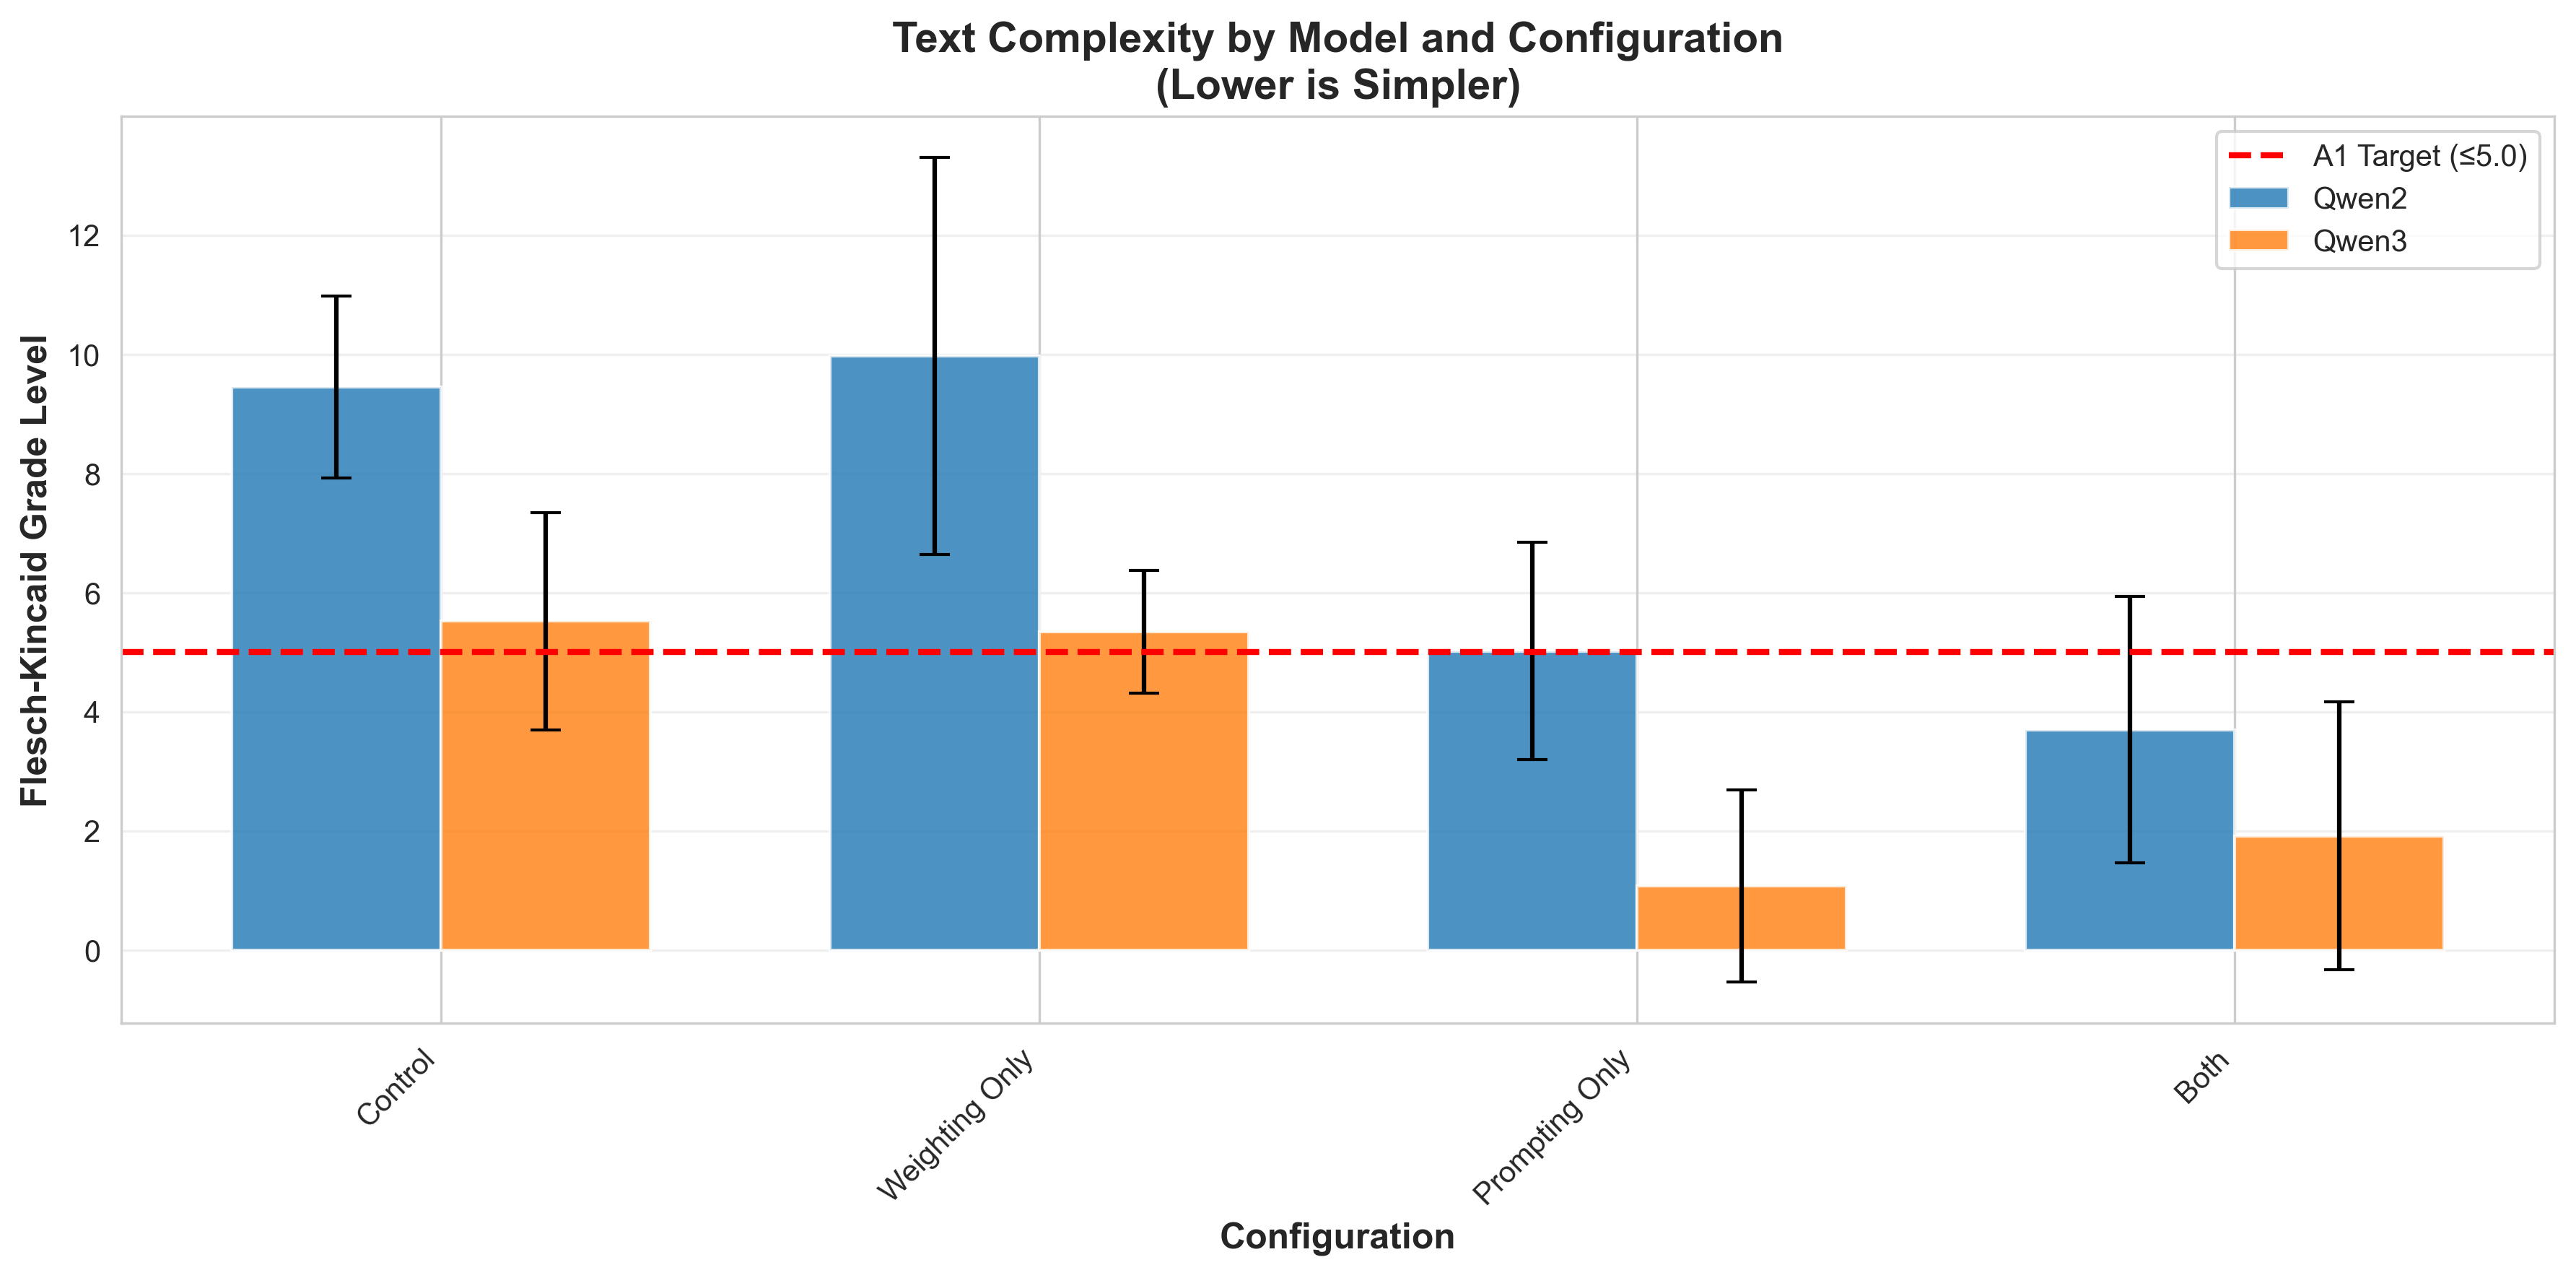
\includegraphics[width=\columnwidth]{figures/model_comparison_fk_grade.png}
% \caption{Flesch-Kincaid Grade Level by model and configuration. Error bars show standard deviation. Horizontal line indicates A1 target (FK ≤ 5.0).}
% \label{fig:model-comparison}
% \end{figure}

\textbf{Key findings:} [TBD pending experiments]

\subsection{Complexity-Speed Trade-offs}

Figure~\ref{fig:tradeoff} visualizes the relationship between text complexity (Flesch-Kincaid Grade) and response time, color-coded by configuration.

% Placeholder for figure
% \begin{figure}[!ht]
% \centering
% 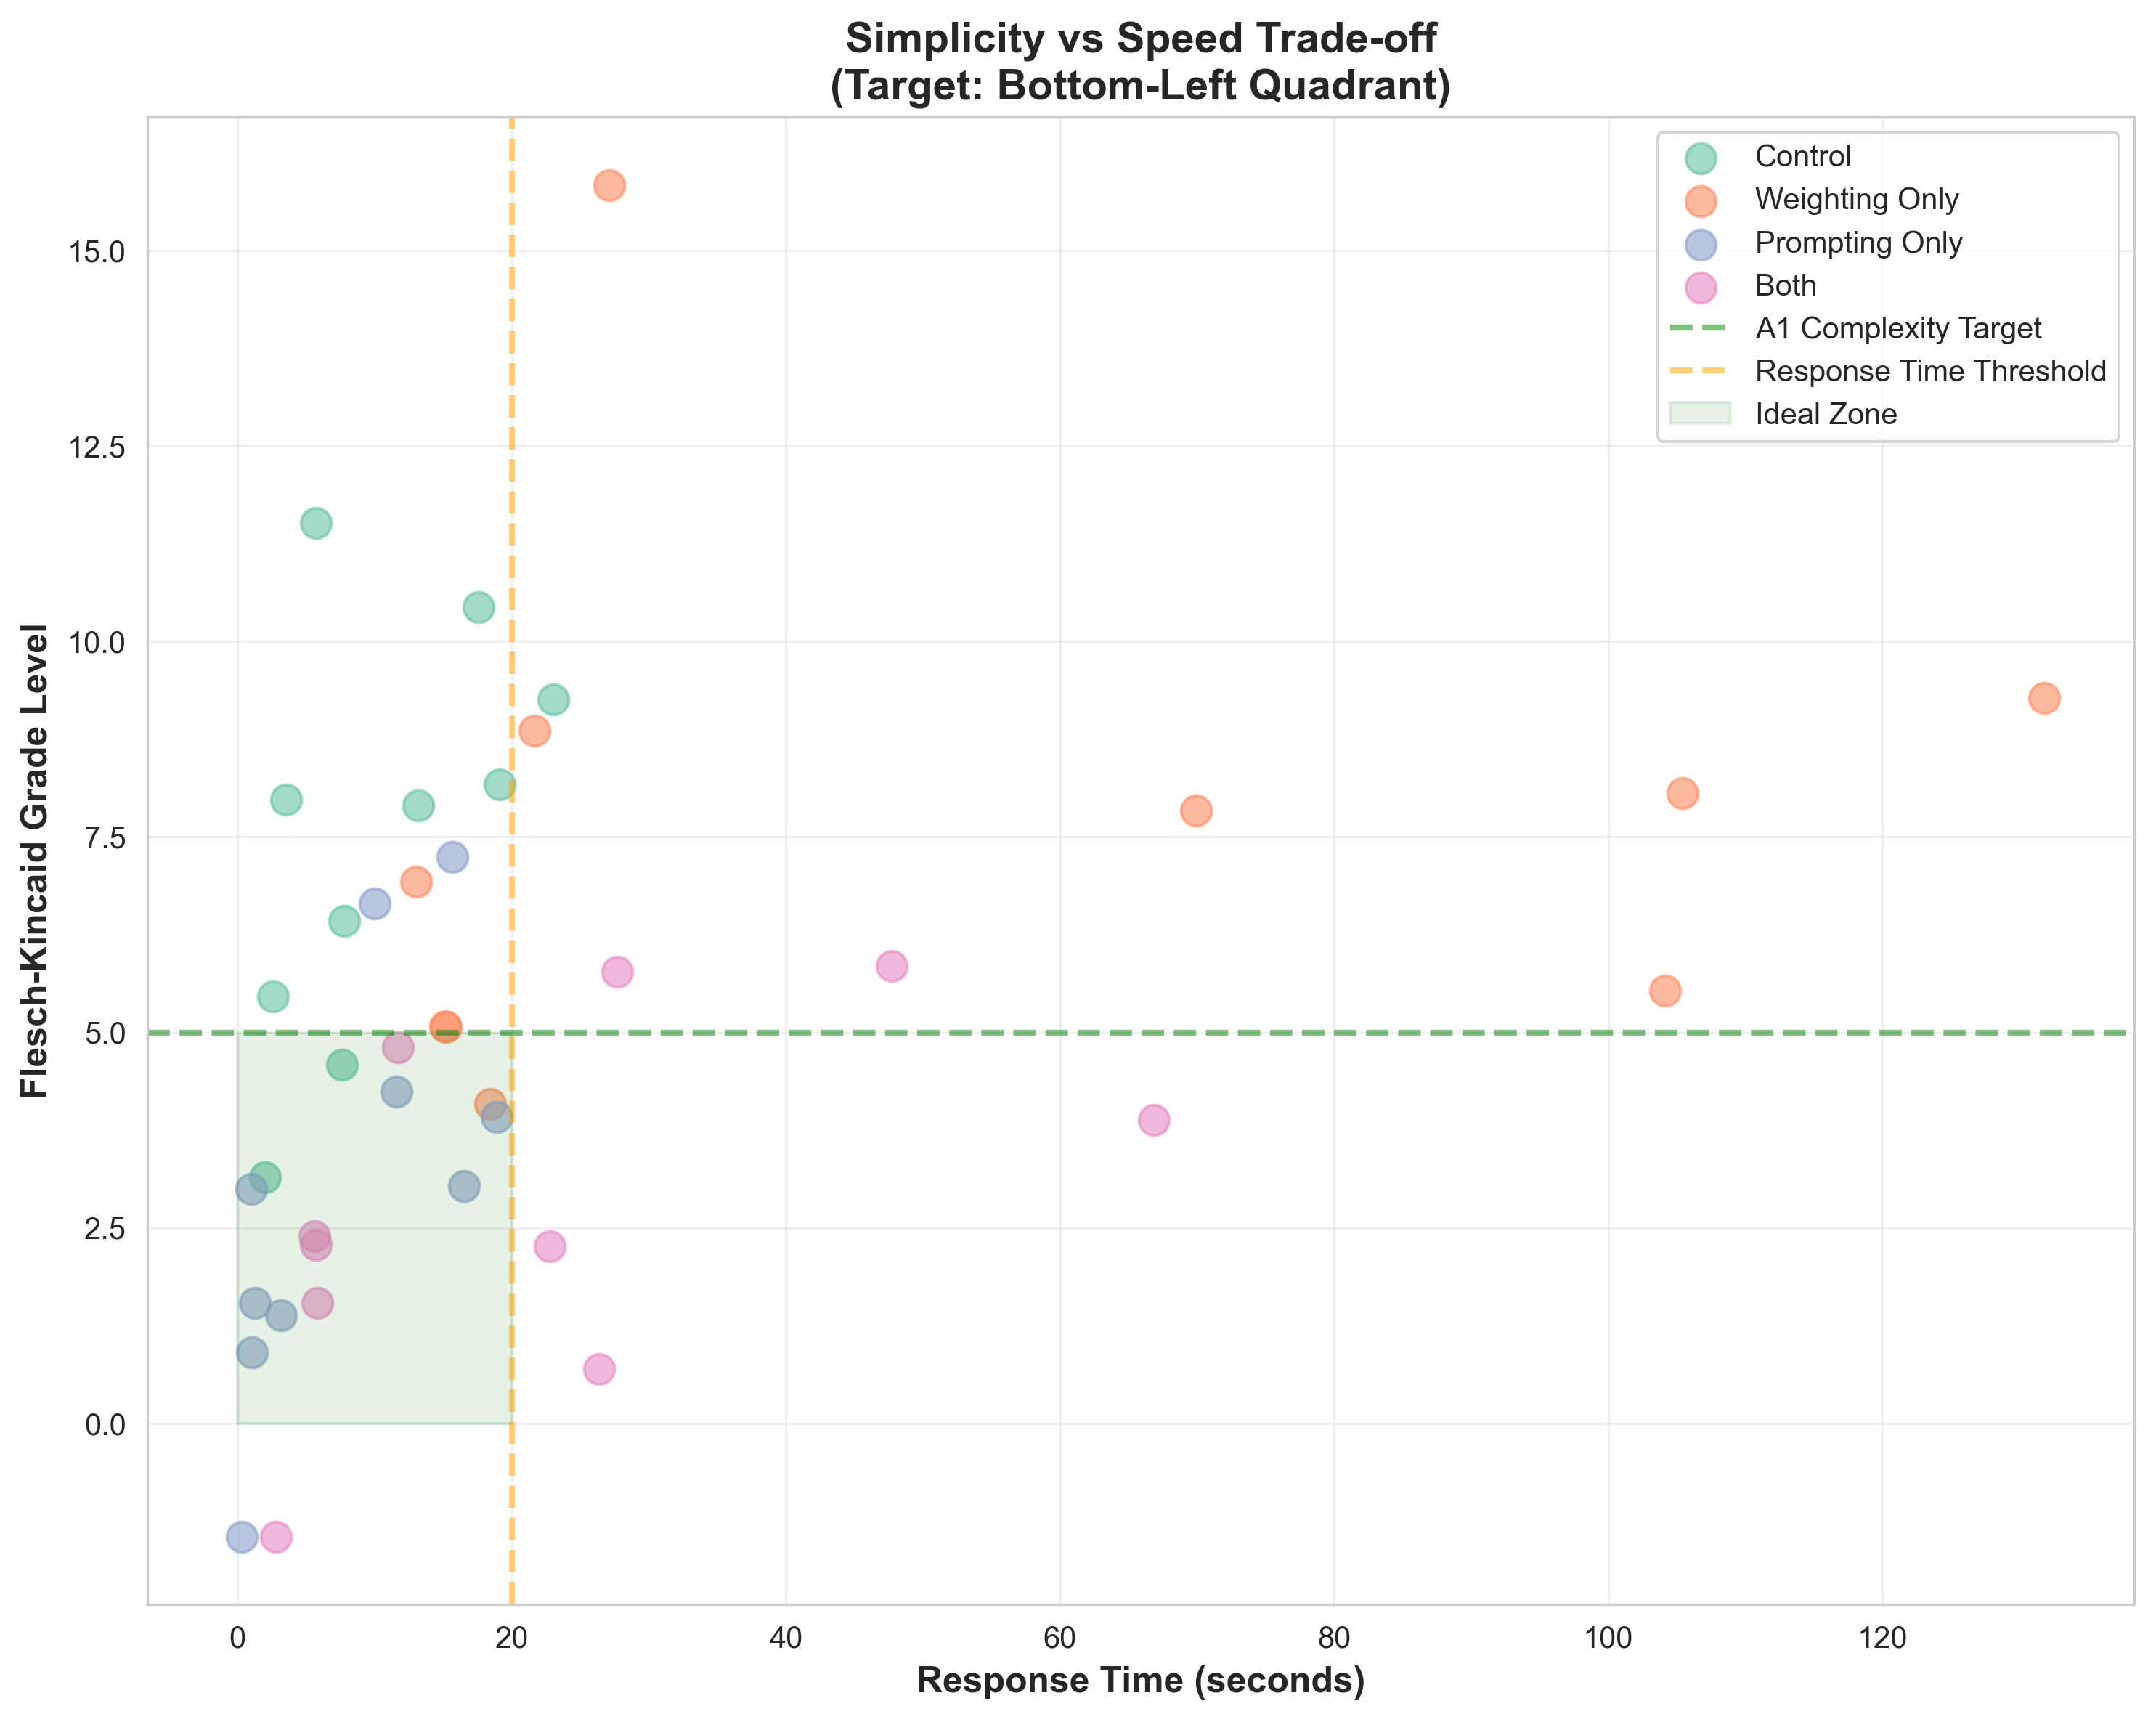
\includegraphics[width=\columnwidth]{figures/complexity_vs_time_tradeoff.png}
% \caption{Complexity-speed trade-off across all observations. Each point represents one model-configuration combination. Shaded region indicates ideal zone (simple + fast).}
% \label{fig:tradeoff}
% \end{figure}

\textbf{Key findings:} [TBD pending experiments]

\subsection{Effect Sizes}

Table~\ref{tab:effect-sizes} reports effect sizes for each intervention across models.

\begin{table*}[!ht]
\centering
\small
\begin{tabular}{lllccc}
\hline
\textbf{Model} & \textbf{Config} & \textbf{FK Grade} & \textbf{Change (\%)} & \textbf{Cohen's d} & \textbf{Flesch Ease} \\
\hline
\multirow{3}{*}{Phi3} & Weighting & TBD & TBD & TBD & TBD \\
& Prompting & TBD & TBD & TBD & TBD \\
& Both & TBD & TBD & TBD & TBD \\
\hline
\multirow{3}{*}{SmolLM} & Weighting & TBD & TBD & TBD & TBD \\
& Prompting & TBD & TBD & TBD & TBD \\
& Both & TBD & TBD & TBD & TBD \\
\hline
\multicolumn{6}{l}{\textit{[Additional models omitted for space]}} \\
\hline
\end{tabular}
\caption{Effect sizes of interventions relative to control baseline. Change (\%) shows percent reduction in FK Grade. Cohen's d quantifies standardized effect size.}
\label{tab:effect-sizes}
\end{table*}

\section{Discussion}

\subsection{Effectiveness of Interventions}

\textbf{Prompting effectiveness:} [TBD: Discuss whether prompting alone achieves A1 targets, explain mechanism (holistic control of vocabulary + sentence structure), compare to prior work on instruction-following in small models]

\textbf{Weighting effectiveness:} [TBD: Discuss whether probability weighting reduces complexity, potential issue of compensatory verbosity (longer sentences with simpler words), comparison to hard constraints in \citet{Li2024}]

\textbf{Synergistic effects:} [TBD: Analyze whether combined interventions outperform individual ones, quantify interaction effect from ANOVA, discuss trade-offs with response time]

\subsection{Model-Specific Findings}

[TBD: Compare models on baseline complexity, responsiveness to interventions, latency characteristics; discuss implications of model size (33M vs 3.8B) on controllability; architectural differences that may affect instruction-following]

\subsection{Practical Implications}

Based on our findings, we offer the following recommendations for deploying small language models in educational applications:

\textbf{For latency-critical applications:} [TBD: Recommend prompting-only if it suffices]

\textbf{For maximum simplicity:} [TBD: Recommend combined interventions if trade-off justified]

\textbf{Model selection:} [TBD: Recommend specific model based on complexity-speed-size trade-offs]

\subsection{Comparison to Prior Work}

Our approach differs from MCTune \citep{Nguyen2024} in flexibility and resource requirements. While MCTune requires fine-tuning LLaMA2-7B on instruction-tuning datasets, our interventions apply at inference time to any pre-trained model. This enables:

\begin{itemize}
\item \textbf{Dynamic adjustment:} Complexity can be modulated per request
\item \textbf{Model portability:} Works across architectures without retraining
\item \textbf{Lower cost:} No compute or data requirements beyond inference
\end{itemize}

However, fine-tuning may achieve more precise control by encoding complexity preferences directly into model weights. Future work should compare both approaches directly.

Our soft vocabulary constraints differ from the hard lexical constraints in \citet{Li2024}. Their Divide and Conquer strategy ensures specific words appear in outputs, while our probability weighting merely increases the likelihood of simpler words. This preserves generation flexibility but may be less effective for strict vocabulary requirements.

\section{Limitations}

\textbf{Sample size:} Our current experiment uses 8 prompts per model. While this yields 192 total observations, larger prompt sets (50+) would improve statistical power for per-model analyses.

\textbf{Prompt dependency:} Results may vary with different prompt types. Our current set focuses on vocabulary and grammar questions; conversation scenarios and error correction may behave differently.

\textbf{No human validation:} Readability formulas are proxies for comprehension, not direct measurements. Validation with A1 learners is necessary to confirm ecological validity.

\textbf{Weight factor not optimized:} We use a fixed 2.0× weight factor. Systematic hyperparameter search (grid search over 1.1-3.0) may identify better values balancing simplicity and fluency.

\textbf{Subword tokenization effects:} Vocabulary words split into subword tokens receive unintended weighting. For example, weighting ``angry'' boosts both ``ang'' and ``ry'', affecting words like ``every'' and ``library''. Whole-word-only weighting strategies may mitigate this.

\textbf{No semantic validation:} We measure complexity but not correctness. Simpler text might sacrifice accuracy (e.g., omitting important details). QA benchmarks should assess semantic preservation.

\textbf{Single language:} English only. Generalization to other L2 contexts (Spanish, French, etc.) requires empirical validation.

\section{Future Work}

\textbf{Immediate extensions:}
\begin{itemize}
\item Expand to 50+ prompts across diverse categories (conversation, cultural topics, error correction)
\item Hyperparameter optimization: grid search for optimal weight factor
\item Human evaluation with 20-30 A1 learners rating comprehensibility and helpfulness
\item Multi-turn dialogue testing for context coherence
\end{itemize}

\textbf{Medium-term research:}
\begin{itemize}
\item Fine-tuning baseline: compare fine-tuned model (no interventions) vs base model (with interventions)
\item Dynamic vocabulary adaptation: expand word list as learners progress (A1 → A2)
\item Cross-linguistic validation: test on Spanish, French, Mandarin learners
\item Semantic correctness: measure factual accuracy with QA benchmarks
\end{itemize}

\textbf{Long-term vision:}
\begin{itemize}
\item Adaptive weighting: learn optimal weight factors per learner via reinforcement learning
\item Multimodal support: integrate images and audio for vocabulary explanations
\item Real-world deployment: pilot with language learning app, measure learning outcomes
\end{itemize}

\section{Conclusion}

We presented the first systematic evaluation of inference-time complexity control for small language models in educational contexts. Through a factorial experiment across 6 models (0.5B-3.8B parameters), we compared context prompting and probability weighting strategies for controlling text complexity for A1 English learners.

Our key contributions include:
\begin{itemize}
\item First comparison of prompting vs probability weighting for complexity control
\item Systematic evaluation across 6 small models suitable for on-device deployment
\item Comprehensive assessment using 18 readability metrics across 192 observations
\item Practical guidelines for deploying language learning assistants
\end{itemize}

[TBD: Final conclusions pending experimental results]

This work demonstrates that small language models can be controlled to produce appropriately simple text for beginner learners without fine-tuning, enabling flexible and resource-efficient deployment in educational applications.

\section{Acknowledgements}

[TBD: Acknowledge funding sources, collaborators, and resources]

\section{Ethical Considerations}

This research focuses on improving educational accessibility for language learners. Potential considerations include:

\begin{itemize}
\item \textbf{Over-simplification:} Excessive simplification may patronize adult learners or omit important information
\item \textbf{Accuracy trade-offs:} Simpler language should not sacrifice factual correctness
\item \textbf{Bias in vocabulary lists:} A1 word lists designed for children may not suit adult learners' interests and needs
\item \textbf{Privacy:} On-device deployment preserves learner privacy by avoiding cloud-based processing
\end{itemize}

\section{Limitations}

See Section 5 for detailed discussion of experimental limitations.

\section{Bibliographical References}\label{sec:reference}

% Placeholder references - replace with actual bibliography
\begin{thebibliography}{99}

\bibitem[Al-Sabbagh and Al-Khalifa(2023)]{Al-Sabbagh2023}
Al-Sabbagh, R. and Al-Khalifa, H. (2023).
\newblock Multi-level text simplification systems: A review.

\bibitem[Al-Thanyyan and Azmi(2020)]{Al-Thanyyan2020}
Al-Thanyyan, S. and Azmi, A. (2020).
\newblock Automated text simplification: A survey.

\bibitem[Albinhassan et al.(2025)]{Albinhassan2025}
Albinhassan, M., et al. (2025).
\newblock Learning and enforcing context-sensitive control for LLMs.
\newblock In \textit{ACL 2025 Student Research Workshop}.

\bibitem[Baez and Saggion(2023)]{Baez2023}
Baez, S. and Saggion, H. (2023).
\newblock LSLlama: Fine-tuning LLaMA for lexical simplification.

\bibitem[Claridge(2005)]{Claridge2005}
Claridge, C. (2005).
\newblock Analysing word frequency in graded readers.

\bibitem[Crossley et al.(2011)]{Crossley2011}
Crossley, S., et al. (2011).
\newblock Text simplification and comprehensible input for L2 learners.

\bibitem[Gala et al.(2018)]{Gala2018}
Gala, N., et al. (2018).
\newblock Simplified texts improve reading fluency in beginning readers.

\bibitem[Li et al.(2024)]{Li2024}
Li, X., et al. (2024).
\newblock Control large language models via divide and conquer.
\newblock In \textit{EMNLP 2024}.

\bibitem[Nguyen et al.(2024)]{Nguyen2024}
Nguyen, T., et al. (2024).
\newblock Multi-control tuning for large language models.
\newblock In \textit{ACL 2024 Findings}.

\bibitem[Raspanti et al.(2025)]{Raspanti2025}
Raspanti, G., et al. (2025).
\newblock Grammar-constrained decoding makes LLMs better logical parsers.
\newblock In \textit{ACL 2025 Industry Track}.

\bibitem[Wang et al.(2025)]{Wang2025}
Wang, Y., et al. (2025).
\newblock CogSteer: Cognition-inspired selective layer intervention.
\newblock In \textit{ACL 2025 Findings}.

\bibitem[Zhang et al.(2025)]{Zhang2025}
Zhang, L., et al. (2025).
\newblock Generation with concept activation vector (GCAV).
\newblock \textit{arXiv:2501.05764}.

\end{thebibliography}

\appendix

\section{Appendix A: Experimental Prompts}

The following 8 prompts were used in our experiments:

\begin{enumerate}
\item What does the word ``library'' mean?
\item Can you explain the difference between ``big'' and ``large''?
\item How do I use ``have'' and ``has'' correctly?
\item What is a simple way to introduce myself in English?
\item Tell me about common breakfast foods.
\item What does ``happy'' mean and when do we use it?
\item How do I ask for directions to the park?
\item Explain what a ``teacher'' does.
\end{enumerate}

\section{Appendix B: Vocabulary List Details}

Our A1 vocabulary list is derived from the Cambridge English Starters curriculum, filtered to remove:
\begin{itemize}
\item Proper nouns (names, places)
\item Numbers and dates
\item Specialized terms (measurement units, technical vocabulary)
\end{itemize}

Final list: 493 words from original 511-word Starters vocabulary.

Example words: \textit{apple, book, cat, dog, eat, friend, go, happy, is, jump, know, like, make, new, open, play, quiet, run, see, talk, under, very, walk, yes, zoo}

\end{document}

